\chapter{Gravitational collapse and the large-scale structure of the universe}

In the previous lectures our study of cosmology has been restricted by the assumptions of homogeneity and isotropy, as stated in the cosmological principle. We know, however, that the cosmological principle is an approximate law. At present times, the universe is homogeneous and isotropic only on distance scales larger than of order 100 Mpc. However, we will see that there is strong evidence that the early universe was very homogeneous and isotropic on all scales, not just on sufficiently large scales. It follows that as the universe evolved, it experienced a loss of homogeneity on small scales. The goal of this lecture is to study the mechanism responsible for this loss of homogeneity, namely gravitational collapse.

\section{Large-scale structure}

Before beginning our study of gravitational collapse, we will discuss in this section the large-scale structure of the universe. As we briefly mentioned in chapter 6, structure formation is the phase in the thermal history of the universe in which the matter (which, after recombination, is composed of neutral atoms and dark matter) begins to form lumps of gas as a result of gravity. These lumps grow larger and denser as the universe evolves, eventually forming the first stars and galaxies. Our discussion of structure formation will be very qualitative, as many of the details of this phase are not yet fully understood, although a lot of progress has been made during the last decade with the help of powerful computer simulations.

The cosmic microwave background (CMB) gives us a snapshot of the universe when it had an age of $t_{\mathrm{rec}}\approx 380,000$ years (with a corresponding redshift of $z_{\mathrm{rec}}\approx1100$). By observing the temperature of the CMB as a function of the direction in the sky, cosmologists have been able to conclude that, at the time of recombination, the universe was homogeneous {\it on all scales} to one part in $10^5$. This statement can be written as follows:
\begin{equation} \label{eq:cmb_densitybound}
\left| \frac{\rho_r(\mathbf{r},t_{\mathrm{rec}})-\bar{\rho}_r(t_{\mathrm{rec}})}{\bar{\rho}_r(t_{\mathrm{rec}})} \right| \lesssim 10^{-5}.
\end{equation}
Here $\rho_r(\mathbf{r},t_{\mathrm{rec}})$ denotes the photon energy density as a function of position $\mathbf{r}$ evaluated at the time of recombination, $t=t_{\mathrm{rec}}$, whereas $\bar{\rho}_r(t_{\mathrm{rec}})$ denotes the average of $\rho_r(\mathbf{r},t_{\mathrm{rec}})$ over all space. What equation (\ref{eq:cmb_densitybound}) shows is that the difference between the actual density and the average density is never larger than $10^{-5}$ times the average density. In other words, the departure from perfect homogeneity (in which case we would have $\rho_r(\mathbf{r},t_{\mathrm{rec}})=\bar{\rho}_r(t_{\mathrm{rec}})$ for all $\mathbf{r}$) is never larger than about one part in $10^5$. The universe was therefore very homogeneous on all scales during the time of recombination.

Today the universe is also very homogeneous, but only on distance scales of order 100 Mpc and larger. On smaller scales we observe {\it structures}, which range from planets and stars to galaxy clusters and superclusters. The structures that are relevant to astrophysics and cosmology are shown in the following table:
\begin{table}[ht]
\begin{center}
\begin{tabular}{p{5cm} l l} \hline\hline
Structures & Scales  \\ \hline
Planets & $10^4-10^5$ km \\
Stars & $10^6-10^8$ km \\
Stellar clusters & $10-100$ pc \\
Galaxies & $1-100$ kpc \\
Galaxy clusters & $1-10$ Mpc \\
Galaxy superclusters & $50-100$ Mpc \\ \hline\hline
\end{tabular}
\end{center}
\end{table}

Galaxy clusters are collections of a few hundreds of galaxies, while galaxy superclusters are collections of several clusters of galaxies. Of course, there exist all kinds of structures smaller than planets (mountains, rocks, cells, etc.), but the important point is that we do not observe structures larger than galaxy superclusters. As we will see in a later lecture, this observation provides an important constraint on the nature of dark matter. In the following we will briefly study the main properties of clusters and superclusters of galaxies.

\subsubsection{Galaxy clusters}

Galaxy clusters are groups of galaxies interacting gravitationally. Most clusters contain a few hundreds of galaxies, although some may contain as few as 100 galaxies or less while the largest ones contain as many as 1000 galaxies or more.\footnote{Collections of 50 or less galaxies are usually classified as galaxy groups.} The total mass of a typical cluster ranges from $10^{14}$ to $10^{15}$ solar masses, of which only about $3\%$ is contained in galaxies (although this number may be larger for small clusters and galaxy groups). The rest of the mass is contained in the intergalactic gas (about $12\%$) and in the dark matter (about $85\%$). The average speeds of the galaxies in clusters (measured with respect to the center of mass of the cluster) are in the order of $1000$ km/s (for comparison, the speed of the Sun relative to center of the Milky Way is around $220$ km/s).
\begin{figure}[ht]
\begin{center}
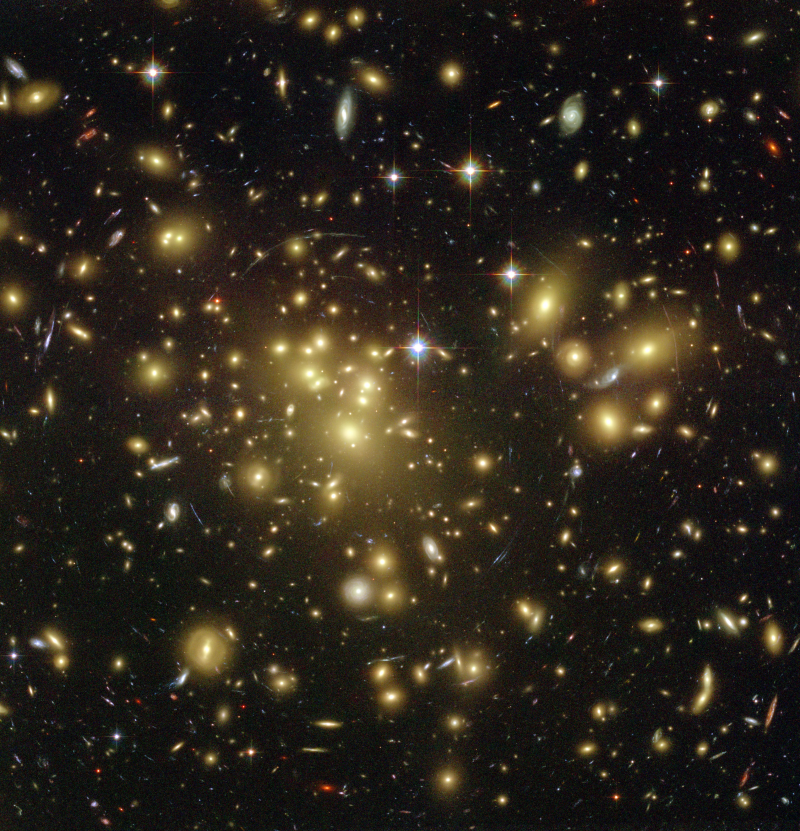
\includegraphics[scale=1.2]{Draw/lec8_1.png}
\end{center}
\caption{Galaxy Cluster Abell 1689 (Image credit: HST, H.\ Ford, JHU)}
\label{fig:lec8_1}
\end{figure}

An important property is that galaxy clusters are in {\it virial equilibrium}. A system in virial equilibrium is one which is neither contracting nor expanding, and which satisfies the virial theorem:
\begin{equation} \label{eq:virial_thm}
\langle E_{\mathrm{pot}}\rangle +2\langle E_{\mathrm{kin}}\rangle =0.
\end{equation}
In this equation $\langle E_{\mathrm{pot}}\rangle$ denotes the average potential energy of the cluster. Since galaxy clusters have roughly spherical shapes (there are exceptions though), we can in general write
\begin{equation} \label{eq:avg_epot}
\langle E_{\mathrm{pot}}\rangle = -\alpha \frac{GM^2}{R},
\end{equation}
where $G$ is Newton's gravitational constant, $M$ is the total mass of the cluster, and $R$ is the radius of the cluster; $\alpha$ is a dimensionless constant of order 1, whose precise value depends on the mass distribution of the cluster.\footnote{As an example, a uniform sphere of mass $M$ and radius $R$ would have $\alpha=3/5$.} On the other hand, $\langle E_{\mathrm{kin}}\rangle$ denotes the average kinetic energy of the cluster, which is given by
\begin{equation} \label{eq:avg_ekin}
\langle E_{\mathrm{kin}}\rangle = \frac{1}{2}M\langle v^2\rangle,
\end{equation}
where $\langle v^2\rangle$ is the average squared speed of the galaxies in the cluster.

If we apply the virial theorem (\ref{eq:virial_thm}), using eqs.\ (\ref{eq:avg_epot}) and (\ref{eq:avg_ekin}), we obtain
\begin{equation}
-\alpha \frac{GM^2}{R}+M\langle v^2\rangle=0,
\end{equation}
\begin{equation}
\Rightarrow~~~~ M=\frac{\langle v^2\rangle R}{\alpha G}.
\end{equation}
This last result is very useful, as it provides a formula for computing the total mass of the cluster, $M$, from the knowledge of $\langle v^2\rangle$, $R$, and $\alpha$. The average squared speed $\langle v^2\rangle$ can be measured directly by observing the Doppler redshift in the emission spectra of the galaxies in a cluster. Similarly, the radius $R$ of a cluster can be measured directly as long as the cluster is not too distant. The constant $\alpha$ is difficult to measure in general, but since we know that it is always of order 1, its precise value is not needed in order to get a rough estimate for the mass $M$.

\subsubsection{Galaxy superclusters}

Galaxy superclusters are collections of several (roughly between 5 and 15) rich clusters of galaxies, plus several dozens of galaxy groups.\footnote{The Local Group (the galaxy group that contains the Milky Way) is part of the Virgo supercluster.} Typical sizes are between 50 and 100 Mpc, although the largest ones can extend to around 200 Mpc. The average separation between superclusters is about 150 Mpc, which has the same order of magnitude of the size of a typical supercluster.\footnote{Compare this fact with the case of stars: the average separation between stars in a galaxy is of order $10^{13}$ km, while the typical size of a star is around $10^6$ km.} The regions between superclusters, which contain very few galaxies, are known as {\it voids}.

Superclusters are {\it not} in virial equilibrium. This is because superclusters are currently undergoing gravitational collapse, meaning that they are still in the process of forming. This is in contrast to galaxy clusters, most of which have finished forming at the present time, and have subsequently achieved virial equilibrium. A useful timescale to distinguish the different structures in the universe is the {\it virialization time}, which is the time lapse from the beginning of gravitational collapse to the time when the system achieves virial equilibrium. The following table shows the virialization times for the large-scale structures:
\begin{table}[ht]
\begin{center}
\begin{tabular}{p{5cm} l l} \hline\hline
Structures & Virialization time  \\ \hline
Galaxies & $10^8$ years \\
Galaxy clusters & $10^9$ years \\
Galaxy superclusters & $10^{10}-10^{11}$ years \\ \hline\hline
\end{tabular}
\end{center}
\end{table}

Comparing these times with the age of the universe ($1.4\times10^{10}$ years), we understand why superclusters are still, at the present time, undergoing gravitational collapse: they simply have not had enough time to achieve a state of virial equilibrium.

The fact that galaxy superclusters are still under formation implies that they can have quite irregular shapes. Unlike galaxy clusters, most of which (especially the rich ones) have roughly spherical shapes, superclusters can have spherical, elongated (filaments), or flattened (walls) shapes. These irregularities give rise to a web-like structure of the universe on its largest scales (fig.\ \ref{fig:lec8_2}).
\begin{figure}[ht]
\begin{center}
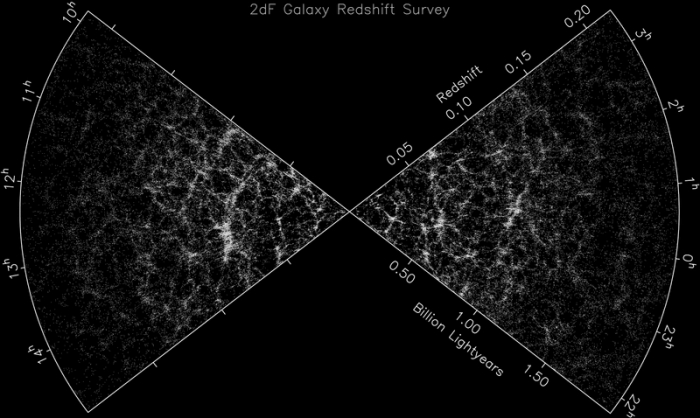
\includegraphics[scale=0.4]{Draw/lec8_2.png}
\end{center}
\caption{The large-scale structure of the universe (Image credit: 2dF Galaxy Redshift Survey)}
\label{fig:lec8_2}
\end{figure}


\section{Gravitational collapse}

We have seen that at the end of recombination the energy content of the universe is formed by neutral particles only: photons, neutrinos, dark matter, and baryonic matter in the form of neutral atoms.\footnote{Dark energy does not play an important role until much later times.} The subsequent evolution is different for each of these four particle species. In this section we will focus on the evolution of the baryonic matter density, but we will comment on what happens to the other species at the end of the section.

After recombination, the initial inhomogeneities in the baryonic matter begin to grow as a result of gravity. Since the gravitational attraction is stronger for larger densities, initially overdense regions start drawing matter from underdense regions. This has the consequence that the density in overdense regions increases in time, while the density in underdense regions decreases in time (see fig.\ \ref{fig:lec8_3}). This is the essence of gravitational collapse.
\begin{figure}[ht]
\begin{center}
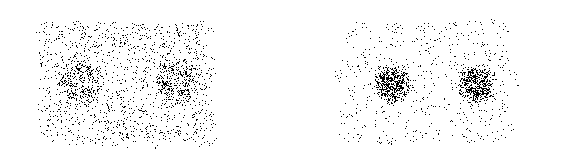
\includegraphics[scale=0.8]{Draw/lec8_3.png}
\end{center}
\caption{Gravitational collapse}
\label{fig:lec8_3}
\end{figure}

Our goal in this section is to describe gravitational collapse in a mathematical way. To do this, we begin by defining the {\it density fluctuation} as follows:
\begin{equation} \label{eq:dens_fluct}
\delta(\mathbf{r},t)=\frac{\rho(\mathbf{r},t)-\bar{\rho}(t)}{\bar{\rho}(t)},
\end{equation}
where $\rho(\mathbf{r},t)$ denotes the mass density of the matter as a function of position $\mathbf{r}$ and time $t$, and $\bar{\rho}(t)$ denotes the average of $\rho(\mathbf{r},t)$ over space.\footnote{We could have also defined $\rho(\mathbf{r},t)$ as the energy density of the baryonic matter, since for nonrelativistic matter the only difference between mass density and energy density is a factor of $c^2$, which would cancel in eq.\ (\ref{eq:dens_fluct}).} An overdense region is one where the local density is larger than the average density, and so $\delta(\mathbf{r},t)>0$ in such a region. Similarly, an underdense region is one where the local density is smaller than the average density, meaning that $\delta(\mathbf{r},t)<0$.

Let us consider a spherical region that is small enough so that we can approximate it as being homogeneous (see fig.\ \ref{fig:lec8_4}). This means that, in this region, we can approximate $\rho(\mathbf{r},t)\approx \rho(t)$, which also implies that $\delta(\mathbf{r},t)\approx \delta(t)$. We will further assume that the rate at which $\delta(t)$ changes in time is much larger than the rate at which the average density $\bar{\rho}(t)$ changes (this is equivalent to neglecting the effects of the Hubble expansion; we will consider these effects later). This means that we can approximate the average density to be constant in time, $\bar{\rho}(t)\approx \bar{\rho}$.
\begin{figure}[ht]
\begin{center}
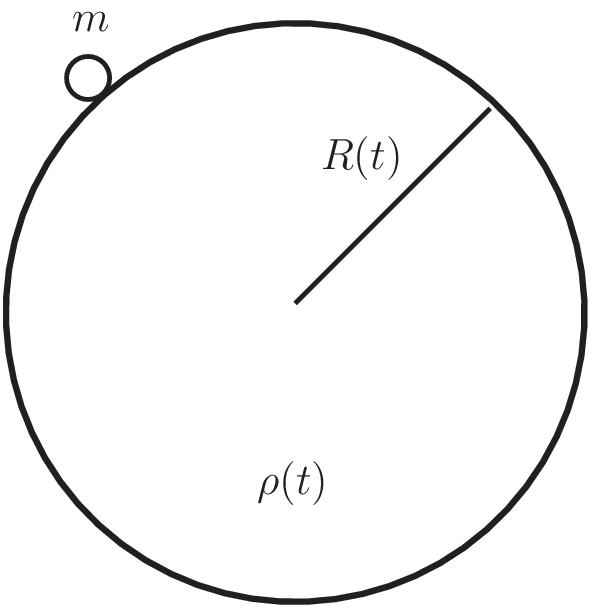
\includegraphics[scale=0.3]{Draw/lec8_4.png}
\end{center}
\caption{Gravitational collapse}
\label{fig:lec8_4}
\end{figure}

Let the mass of the spherical region be $M$, and let its radius be $R(t)$ (which changes in time as a result of gravitational collapse). Consider a small particle of mass $m$ on the boundary of the spherical region. The force felt by the particle is given by Newton's gravitational law:
\begin{equation} \label{eq:force1}
F=-\frac{G(\Delta M)m}{R(t)^2},
\end{equation}
where $\Delta M$ is the excess mass of the sphere relative to the medium, that is,
\begin{equation}
\begin{split}
\Delta M&=\left(\rho(t)-\bar{\rho}\right)V(t)\\
&=\left(\frac{\rho(t)-\bar{\rho}}{\bar{\rho}}\right)\bar{\rho}\left(\frac{4\pi}{3}R(t)^3\right)\\
&=\frac{4\pi}{3}\bar{\rho} R(t)^3\delta(t),
\end{split}
\end{equation}
where $V(t)$ is the volume of the spherical region, and in the last line we used eq.\ (\ref{eq:dens_fluct}). Notice that the position of the particle relative to the center of the sphere is precisely $R(t)$, and so the acceleration of the particle equals $\ddot{R}(t)$, the second time derivative of $R(t)$. By Newton's second law we then have that the force on the particle is given by
\begin{equation} \label{eq:force2}
F=m\ddot{R}(t).
\end{equation}
Combining eqs.\ (\ref{eq:force1}) and (\ref{eq:force2}) we obtain
\begin{equation}
m\ddot{R}(t)=-\frac{Gm}{R(t)^2}\left(\frac{4\pi}{3}\bar{\rho}R(t)^3\delta(t)\right),
\end{equation}
\begin{equation} \label{eq:grav_coll1}
\Rightarrow~~~~ \frac{\ddot{R}(t)}{R(t)}=-\frac{4\pi G\bar{\rho}}{3}\delta(t).
\end{equation}
On the other hand, we know that we can relate the density of the sphere to its radius, since the total mass $M$ is constant. Explicitly, we have
\begin{equation}
\begin{split}
M&= \rho(t)V(t)\\
&=\left(\frac{\left(\rho(t)-\bar{\rho}\right)+\bar{\rho}}{\bar{\rho}}\right)\bar{\rho}\left(\frac{4\pi}{3}R(t)^3\right)\\
&=\frac{4\pi}{3}\bar{\rho} \left(1+\delta(t)\right)R(t)^3,
\end{split}
\end{equation}
\begin{equation}
\Rightarrow~~~~ R(t)^3=\left(\frac{3M}{4\pi\bar{\rho}}\right)\frac{1}{\left(1+\delta(t)\right)},
\end{equation}
\begin{equation} \label{eq:grav_coll2}
\Rightarrow~~~~ R(t)=\left(\frac{3M}{4\pi\bar{\rho}}\right)^{1/3}\frac{1}{\left(1+\delta(t)\right)^{1/3}}.
\end{equation}
Now, remember that our goal is to study the evolution of inhomogeneities after recombination. From our discussion at the beginning of the lecture, we know that the relative size of these inhomogeneities was very small. In other words, $\delta(\mathbf{r},t)\ll1$ at the early stages of gravitational collapse.\footnote{Of course, eventually $\delta(\mathbf{r},t)$ will become large, which is in fact what we observe at the present time. The analysis in this case becomes much more complicated and is usually studied with the help of computer simulations.} Under this assumption we can approximate
\begin{equation}
\frac{1}{\left(1+\delta(t)\right)^{1/3}}\approx 1-\frac{1}{3}\delta(t).
\end{equation}
(Try to show this if you know about Taylor's theorem.) From eq.\ (\ref{eq:grav_coll2}) we then find the approximate relation
\begin{equation} \label{eq:grav_coll3}
R(t)=\left(\frac{3M}{4\pi\bar{\rho}}\right)^{1/3}\left(1-\frac{1}{3}\delta(t)\right).
\end{equation}
If we now take the second time derivative of this last equation we get
\begin{equation} \label{eq:grav_coll4}
\ddot{R}(t)=-\left(\frac{3M}{4\pi\bar{\rho}}\right)^{1/3}\frac{1}{3}\ddot{\delta}(t).
\end{equation}
From eqs.\ (\ref{eq:grav_coll3}) and (\ref{eq:grav_coll4}) we obtain
\begin{equation}
\begin{split}
\frac{\ddot{R}(t)}{R(t)}&=-\frac{1}{3}\ddot{\delta}(t)\frac{1}{\left(1-\frac{1}{3}\delta(t)\right)}\\
&\approx -\frac{1}{3}\ddot{\delta}(t),
\end{split}
\end{equation}
where the last approximation follows because $\ddot{\delta}(t)$ is already a small quantity, and so we can safely neglect the factor of $\delta(t)$ in the denominator. In other words, we are working to first order in the function $\delta(t)$ and its derivatives. Finally, if we plug the last result into eq.\ (\ref{eq:grav_coll1}) we obtain
\begin{equation}
-\frac{1}{3}\ddot{\delta}(t)=-\frac{4\pi G\bar{\rho}}{3}\delta(t),
\end{equation}
\begin{equation} \label{eq:grav_coll5}
\Rightarrow~~~~ \ddot{\delta}(t)=4\pi G\bar{\rho}\delta(t).
\end{equation}
Eq.\ (\ref{eq:grav_coll5}) is a differential equation for the function $\delta(t)$. Its solution is given by
\begin{equation} \label{eq:delta_sol}
\delta(t)=Ce^{t/t_{\mathrm{dyn}}},
\end{equation}
where $C$ is a constant that has to be computed from the initial conditions, and we defined the {\it dynamical timescale}
\begin{equation}
t_{\mathrm{dyn}}\equiv \frac{1}{\sqrt{4\pi G \bar{\rho}}}.
\end{equation}

%\par\vspace{\baselineskip}
\newpage

{\bf Exercise.}
\begin{itemize}
\item [(a)] Find the second time derivative of $\delta(t)$ from the solution (\ref{eq:delta_sol}), and verify that eq.\ (\ref{eq:grav_coll5}) is satisfied.
\item [(b)] Suppose that the initial value of the density fluctuation is $\delta(t=0)=10^{-3}$. Find the value of $\delta(t)$ at $t=10t_{\mathrm{dyn}}$.
\end{itemize}

\par\vspace{\baselineskip}

Notice that the constant $C$ in eq.\ (\ref{eq:delta_sol}) could be positive or negative. Clearly, $C$ will be positive for an initially overdense inhomogeneity; what eq.\ (\ref{eq:delta_sol}) then tells us is that $\delta(t)$ will always be positive, and that it will grow larger in time. Similarly, for an initially underdense inhomogeneity $C$ will be negative, and so $\delta(t)$ will always be negative and it will grow larger (it will become more negative) in time. This confirms what we qualitatively discussed at the beginning of the section: initially overdense regions become more and more overdense in time, while initially underdense regions become more and more underdense in time.

Another important thing that eq.\ (\ref{eq:delta_sol}) tells us is that $\delta(t)$ will become large on timescales of the order of $t_{\mathrm{dyn}}$. This conclusion has a caveat however, namely that so far we have only considered gravity. But there are two other effects that act {\it against} gravitational collapse: one is the pressure and the other is the Hubble expansion. In the following we will study these effects in order to see how they modify the above conclusions.

\subsection{Effects of pressure}

We have seen that, in the absence of any other effects apart from gravity, matter will tend to collapse exponentially fast. Of course, this is not what we observe; planets, stars, and galaxies, for instance, are perfectly stable systems. There must be some force, then, that opposes gravity in such a way that the net force is zero and the system can remain in stable equilibrium. This force, of course, is provided by the pressure.

Let us consider a spherical cloud of gas with initial radius $R$. As soon as gravitational collapse starts, the gas in the system will attempt to stop the contraction by building up a pressure gradient; it is this gradient that gives rise to an outward-directed force that opposes gravity. As the cloud contracts the gravitational force on each layer becomes stronger, and so the pressure gradient has to become steeper in order to stop the collapse. This steepening of the pressure gradient is not instantaneous however, since the ``news'' about the collapse travel at a finite speed through the gas cloud. This speed is given by the {\it sound speed} $c_s$ of the gas, which corresponds to the speed at which pressure perturbations propagate through a given medium. The typical time it takes for the pressure gradient to become sufficiently steep and stop the collapse is given by the {\it pressure timescale}:
\begin{equation}
t_p\equiv \frac{1}{2\pi}\frac{R}{c_s}.
\end{equation}
Notice that $R/c_s$ is nothing but the time it takes for a pressure perturbation to travel, along a straighy line, from the edge of the cloud to the center. The numerical factor of $1/2\pi$ is not really important, and is a result of the fact that pressure perturbations are waves.

The important question is the following: can the cloud of gas build up a pressure gradient quickly enough to stop the collapse? Clearly, to answer this question we need to compare the pressure timescale, $t_p$, with the dynamical timescale, $t_{\mathrm{dyn}}$. Recall that $t_{\mathrm{dyn}}$ is the typical time it takes for an inhomogeneity to grow large, and so we can identify $t_{\mathrm{dyn}}$ as the time for gravitational collapse. If $t_p>t_{\mathrm{dyn}}$ then the pressure in the gas does not act fast enough to halt the contraction; the collapse will then continue until some new effect happens that makes $t_p$ shorter,\footnote{In the case of stars, this new effect corresponds to nuclear fusion, which provides the pressure needed to stabilize the star against gravity.} or until the cloud becomes so dense that a black hole forms.

To stop the collapse and make the system stable, it is then necessary to have $t_p<t_{\mathrm{dyn}}$. This inequality can be written as follows:
\begin{equation}
\frac{1}{2\pi}\frac{R}{c_s}<\frac{1}{\sqrt{4\pi G \bar{\rho}}},
\end{equation}
which implies an upper bound on the radius $R$ of the gas cloud:
\begin{equation} \label{eq:jeans_def}
R< c_s\left(\frac{\pi}{G\bar{\rho}}\right)^{1/2} \equiv \lambda_J.
\end{equation}
This upper bound, $\lambda_J$, is known as the {\it Jeans length}. From this last result we can state the criterion for gravitational collapse in terms of the size of the system. If $R<\lambda_J$, the collapse will be stopped by the pressure and the system will reach a state of equilibrium. If $R>\lambda_J$, the collapse will continue as described above.

Let us next apply these results to the matter inhomogeneities in the universe. Recombination occurs during the matter-dominated epoch, which implies that we can neglect both the radiation density and the dark energy density in the Friedmann equation:
\begin{equation} \label{eq:fried_eq_inhom}
H^2=\frac{8\pi G}{3}\bar{\rho},
\end{equation}
where $H=\dot{a}/a$ is the Hubble parameter. Notice that the Friedmann equation involves the average density $\bar{\rho}$, not the actual matter density $\rho(\mathbf{r},t)$. This is because the Friedmann equation follows from the Einstein equations under the assumption of perfect homogeneity, and therefore corresponds to the leading-order approximation when we move on to study small inhomogeneities. Solving for $\bar{\rho}$ from eq.\ (\ref{eq:fried_eq_inhom}) we can express the dynamical timescale in terms of the Hubble parameter as follows:
\begin{equation}
\begin{split}
t_{\mathrm{dyn}}&=\frac{1}{\sqrt{4\pi G\bar{\rho}}}\\
&=\sqrt{\frac{2}{3}}\frac{1}{H}.
\end{split}
\end{equation}
Expressing also the Jeans length in terms of $H$ gives
\begin{equation} \label{eq:jeans_hubble}
\lambda_J=2\pi\sqrt{\frac{2}{3}}\frac{c_s}{H}.
\end{equation}
Let us first study gravitational collapse at times before recombination during the matter-dominated epoch. During this stage the baryons (atomic nuclei and electrons) are coupled to the photons in a state of thermal equilibrium. Moreover, even though the universe is matter-dominated at this time, the baryon energy density is smaller than the radiation energy density,\footnote{It is because of the dark matter that the universe is matter-dominated at this time.} which implies that the thermodynamic properties of the cosmic plasma will be approximately those of a gas of photons. Now, one can show that the sound speed of a gas of photons is given by\footnote{You may find surprising that the sound speed of a gas of photons is not exactly $c$, since after all the photons in the gas are all moving at the speed of light. However, remember that the sound speed is the speed at which pressure perturbations travel in a fluid, which in general will be smaller than the average speed of the particles that compose the fluid.
}
\begin{equation}
c_s=\frac{c}{\sqrt{3}}.
\end{equation}
Taking this value as the approximate sound speed of the cosmic plasma before recombination, we find from eq.\ (\ref{eq:jeans_hubble}) a corresponding Jeans length of
\begin{equation}
\lambda_J= \frac{2\pi\sqrt{2}}{3}\frac{c}{H}\approx 3\frac{c}{H}.
\end{equation}
Recall that the size of the observable universe is of the order of the Hubble distance $c/H$. What the above equation tells us is that the Jeans length is larger than the observable universe. Although in the above analysis we concluded that inhomogeneities with sizes larger than $\lambda_J$ will collapse gravitationally, we did not take into account the effects of the expansion of the universe. These effects become dominant over the Newtonian gravitational effects precisely on distance scales of the order of $c/H$ and larger. This implies that an inhomogeneity with size $R>\lambda_J\approx 3c/H$ will not actually undergo gravitational collapse. The important conclusion, then, is that baryon inhomogeneities do not grow before recombination.

Let us next see what happens after recombination. The baryons (which now are in the form of neutral atoms) are now completely decoupled from the photons, so the thermodynamic properties of the baryonic matter are not related to those of the photons, as happened before recombination. One can show that the sound speed of the baryonic matter is now given by
\begin{equation} \label{eq:sound_speed2}
c_s=\left(\frac{k_B T}{\bar{m}}\right)^{1/2},
\end{equation}
where $k_B$ is the Boltzmann constant, $T$ is the temperature, and $\bar{m}$ is the average mass of the particles in the baryonic fluid (which after recombination is approximately equal to $1.22$ times the proton mass). Notice that, since $T$ decreases as the universe expands, so does the sound speed. Evaluating at the time just after the end of recombination, one finds the value $c_s\approx1.5\times10^{-5}c$, which corresponds to a Jeans length of
\begin{equation}
\lambda_J\approx 7.7\times10^{-5}\frac{c}{H}.
\end{equation}
In contrast to what happens before recombination, the Jeans length is now much smaller than the Hubble distance. There exist inhomogeneities, then, with sizes larger than $\lambda_J$ (but smaller than $c/H$, so that the Hubble expansion will not be relevant) that will undergo gravitational collapse. This confirms that structure formation only takes place after the end of recombination, as we stated at the beginning of the lecture.

\subsection{Effects of Hubble expansion}

We have already discussed qualitatively how the expansion of the universe acts against gravitational collapse, and in particular, how it prevents inhomogeneities with sizes larger than the Hubble distance from collapsing. The main conclusion of the previous subsection is that an inhomogeneity of size $R$ will undergo gravitational collapse only if
\begin{equation}
\lambda_J<R<\frac{c}{H}.
\end{equation}
If $R<\lambda_J$ then the pressure in the fluid will halt the collapse. If $R>c/H$ then the Hubble expansion will dominate over the Newtonian gravitational attraction and the collapse will not take place.

Our next goal is to find how the density fluctuation $\delta(t)$ evolves in time. We already did this at the beginning of the section by means of a purely Newtonian analysis, finding that $\delta(t)$ increases exponentially fast; we want to see now how the effects of the expansion of the universe change this picture. For this we need to use the Einstein equations, which become quite complicated after one drops the assumption of perfect homogeneity. One can show that the differential equation that determines $\delta(t)$ (assumed to be small) reads
\begin{equation} \label{eq:delta_eq1}
\ddot{\delta}(t)+2H(t)\dot{\delta}(t)=4\pi G\bar{\rho}(t)\delta(t).
\end{equation}
Notice that for $H=0$, i.e.\ in a static universe, we recover the Newtonian equation (\ref{eq:grav_coll5}) as expected. It is convenient to express the average matter density $\bar{\rho}$ in terms of the matter density parameter $\Omega_m$ as follows:
\begin{equation}
\Omega_m(t)=\frac{\bar{\rho}(t)}{\rho_c(t)}=\frac{8\pi G}{3H(t)^2}\bar{\rho}(t),
\end{equation}
\begin{equation}
\Rightarrow~~~~ 4\pi G\bar{\rho}(t)=\frac{3}{2}\Omega_m(t)H(t)^2.
\end{equation}
Using this in eq.\ (\ref{eq:delta_eq1}) we find
\begin{equation} \label{eq:delta_eq2}
\ddot{\delta}(t)+2H(t)\dot{\delta}(t)-\frac{3}{2}\Omega_m(t)H(t)^2\delta(t)=0.
\end{equation}

Let us first solve eq.\ (\ref{eq:delta_eq2}) for the radiation-dominated epoch. During this time the baryons are coupled to the photons, so the density fluctuation $\delta(t)$ corresponds to the dark matter in this case. In a universe dominated by radiation the contribution of the matter to the total energy is negligible, and so $\Omega_m\approx0$. Also, as it was shown in chapter 5, the Hubble parameter for a radiation-dominated universe is given by
\begin{equation}
H(t)=\frac{1}{2t}.
\end{equation}
With these results eq.\ (\ref{eq:delta_eq2}) reduces to
\begin{equation} \label{eq:delta_eq_rad}
\ddot{\delta}(t)+\frac{1}{t}\dot{\delta}(t)=0.
\end{equation}
This equation has the following solution:
\begin{equation}
\delta(t)=C_1\log t,
\end{equation}
where $C_1$ is a constant. Recall that the logarithm is a function that increases very slowly. The above solution then implies that $\delta(t)$ increases very slowly during the radiation-dominated epoch, and so the gravitational collapse of the dark matter occurs very slowly during this stage.

Next, we solve eq.\ (\ref{eq:delta_eq2}) for the matter-dominated epoch, but before recombination. The density fluctuation $\delta(t)$ again is that of the dark matter, since baryons are strongly coupled to photons in the cosmic plasma. In a universe dominated by matter the contributions of the radiation and dark energy are negligible, and so $\Omega_m\approx 1$. From the results of chapter 5 we also know that the Hubble parameter in a matter-dominated universe is given by
\begin{equation}
H(t)=\frac{2}{3t}.
\end{equation}
Using these results in eq.\ (\ref{eq:delta_eq2}) we find
\begin{equation} \label{eq:delta_eq_mat}
\ddot{\delta}(t)+\frac{4}{3t}\dot{\delta}(t)-\frac{2}{3t^2}\delta(t)=0.
\end{equation}
This equation has the following solution:
\begin{equation}
\delta(t)=C_2t^{2/3},
\end{equation}
where $C_2$ is a constant. This result shows that, after the universe becomes matter-dominated (which, remember, occurs before recombination), dark matter inhomogeneities begin to grow as $\delta(t)\propto t^{2/3}$. Notice that this growth rate is much slower than the exponential rate that we found when neglecting the effects of the Hubble expansion.

\par\vspace{\baselineskip}

{\bf Exercise.} The differential equations (\ref{eq:delta_eq_rad}) and (\ref{eq:delta_eq_mat}) are second order equations (they involve second time derivatives), which means that in fact they have two independent solutions.
\begin{itemize}
\item [(a)] Verify that the general solution of eq.\ (\ref{eq:delta_eq_rad}) is given by
\begin{equation}
\delta(t)=C_1\log t+C_1',
\end{equation}
where $C_1$ and $C_1'$ are arbitrary constants.
\item [(b)] Verify that the general solution of eq.\ (\ref{eq:delta_eq_mat}) is given by
\begin{equation}
\delta(t)=C_2t^{2/3}+C_2'\frac{1}{t},
\end{equation}
where $C_2$ and $C_2'$ are arbitrary constants.
\item [(c)] In the above analysis we did not bother with considering these additional solutions ($C_1'$ in part (a), and $C_2'/t$ in part (b)). Why is this justified?
\end{itemize}

\par\vspace{\baselineskip}

Baryon inhomogeneities do not grow before recombination, as we have seen above. But what happens after recombination? The universe is still matter-dominated, and the baryons are now decoupled from the photons, so one may think that we could apply the above analysis to baryons just like we did to dark matter, and conclude that the baryonic density fluctuation grows proportional to $t^{2/3}$ after recombination. In fact, baryon inhomogeneities begin to grow {\it faster} than $\propto t^{2/3}$ (see fig.\ \ref{fig:lec8_5}). This is because, by the end of recombination, the dark matter inhomogeneities have already grown significantly, and so the atoms that form the baryonic matter are attracted to the dark matter structures that have formed by this time. In other words, in the absence of dark matter, baryonic inhomogeneities would grow slower and, in fact, their size at the present time would be much smaller than what observations suggest. Thus, observations of the large-scale structure of the universe provide an 
independent evidence for the existence of dark matter.
\begin{figure}[ht]
\begin{center}
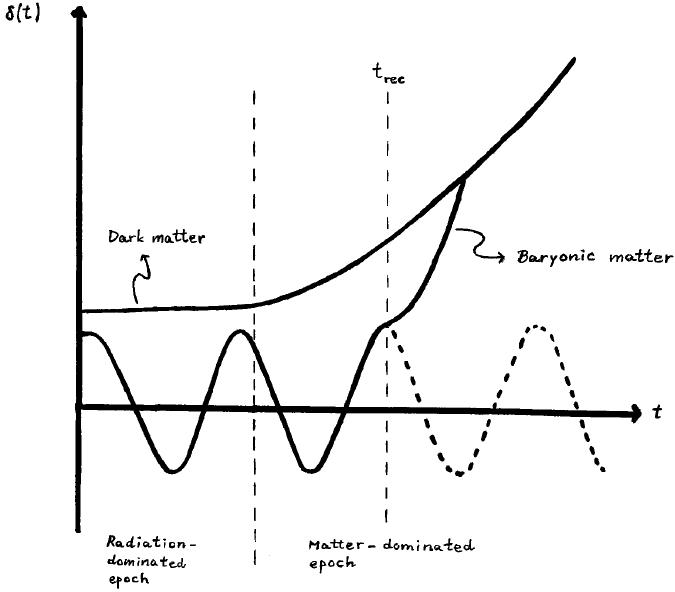
\includegraphics[scale=0.5]{Draw/lec8_5.png}
\end{center}
\caption{Evolution of inhomogeneities}
\label{fig:lec8_5}
\end{figure}

As discussed above, the gravitational collapse may eventually stop due to the effects of pressure. This is in fact what happens to dark matter, which forms the dark matter halos that we (indirectly) observe today around galaxies. Initially, pressure also halts the gravitational collapse of the baryonic matter. However, unlike what happens to dark matter, baryonic matter eventually cools down by emitting radiation. As a consequence, the temperature of a cloud of baryonic gas will decrease in time, and by eq.\ (\ref{eq:sound_speed2}) the sound speed of the gas will decrease as well. Also, we see from eq.\ (\ref{eq:jeans_def}) that the Jeans length will accordingly decrease, which implies that the condition for collapse ($R>\lambda_J$) will eventually be satisfied as the gas continues to cool down. The conclusion is that, for baryonic matter, gravitational collapse will continue until the formation of the first stars takes place.